\documentclass[titlepage]{article}
\usepackage[utf8]{inputenc}
\usepackage{hyperref}
\usepackage{color}
\usepackage{float}
\restylefloat{figure}
\usepackage{subcaption}
\usepackage{amsmath}
\usepackage{amssymb}
\usepackage{minted}
\usepackage{graphicx}
\DeclareGraphicsExtensions{.eps}
\usepackage{fancyhdr}
\pagestyle{fancy}
\lhead{Fractals and the Beauty of Nature}
\author{Chanthosh Sivanandam \\ Erik Andersen \\ Henrik Flindt }
\title{Fractals and the Beauty of Nature \\ DM550 - Fall Project 2017}
\begin{document}
\maketitle
\section{Sierpinski Triangle}
Initially, implementation of the Sierpinski triangle was build upon the idea of placing inverted triangles inside other triangles. It turned out to be a tad complicated, but it yielded some rather interesting results, which can be seen here:
\begin{figure}[H]
  \centering
  \begin{subfigure}[b]{0.4\textwidth}
    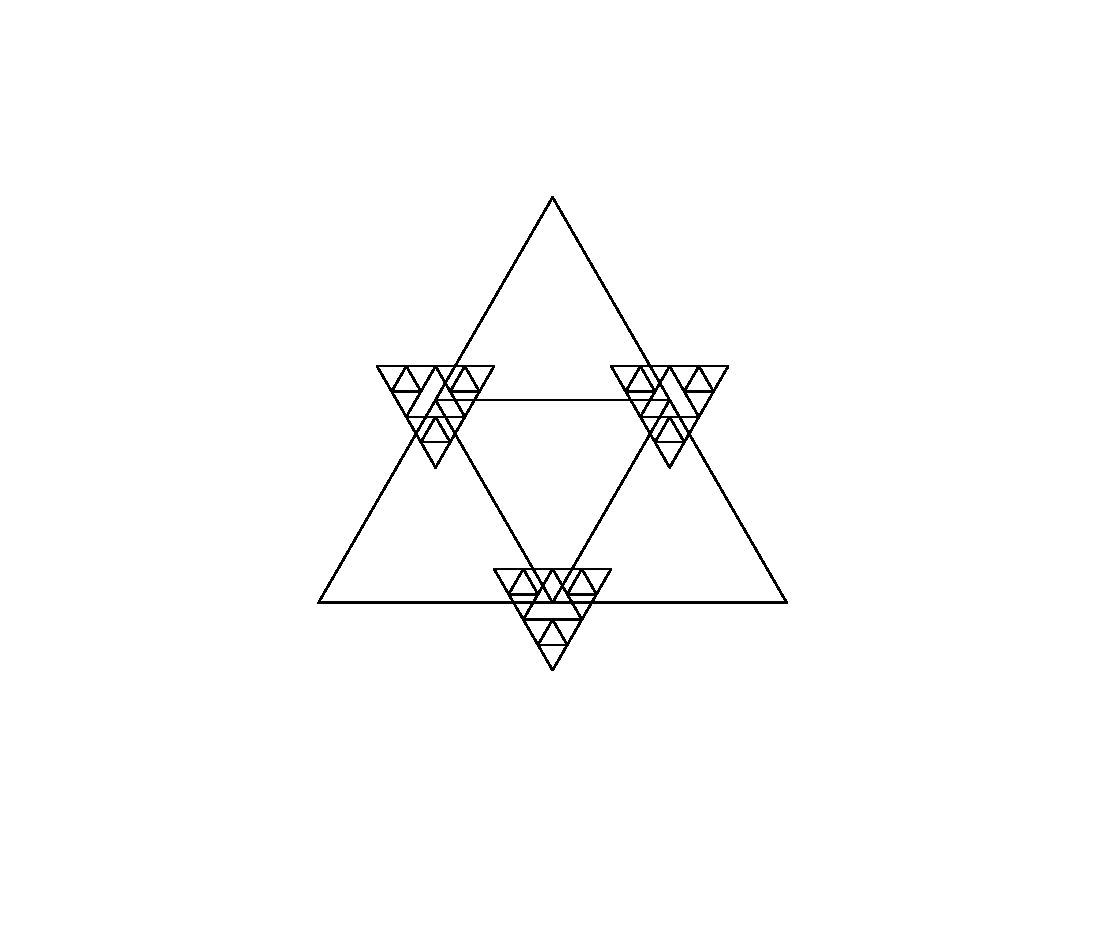
\includegraphics[width=\textwidth]{wrongtriangle}
    \caption{An unsuccessful attempt}
  \end{subfigure}
  \begin{subfigure}[b]{0.5\textwidth}
    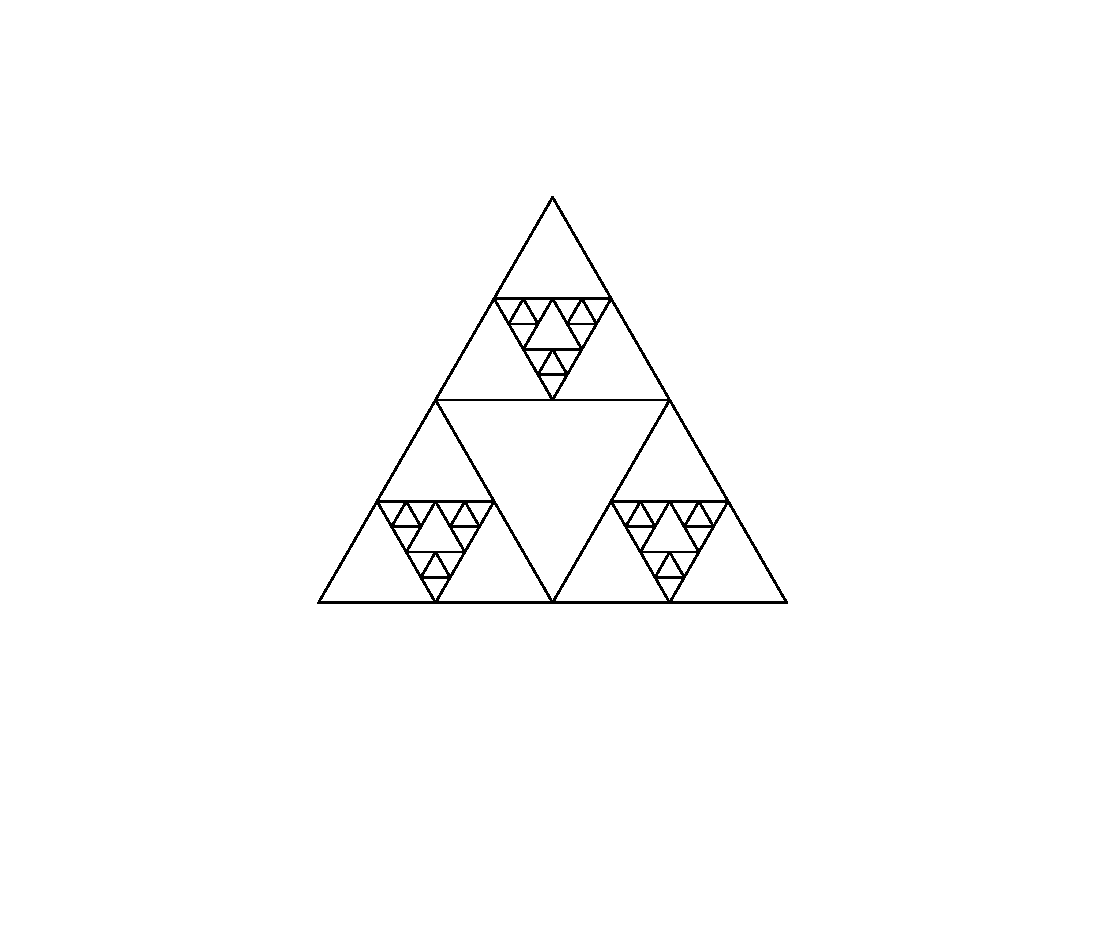
\includegraphics[width=\textwidth]{wrongtriangle2}
    \caption{Another unsuccessful attempt}
  \end{subfigure}
\end{figure}
After meddling around for some time, a decision was made to try the approach suggested in the project description. A successful algorithm that gave the expected result was then rapidly developed.
\begin{figure}[H]
  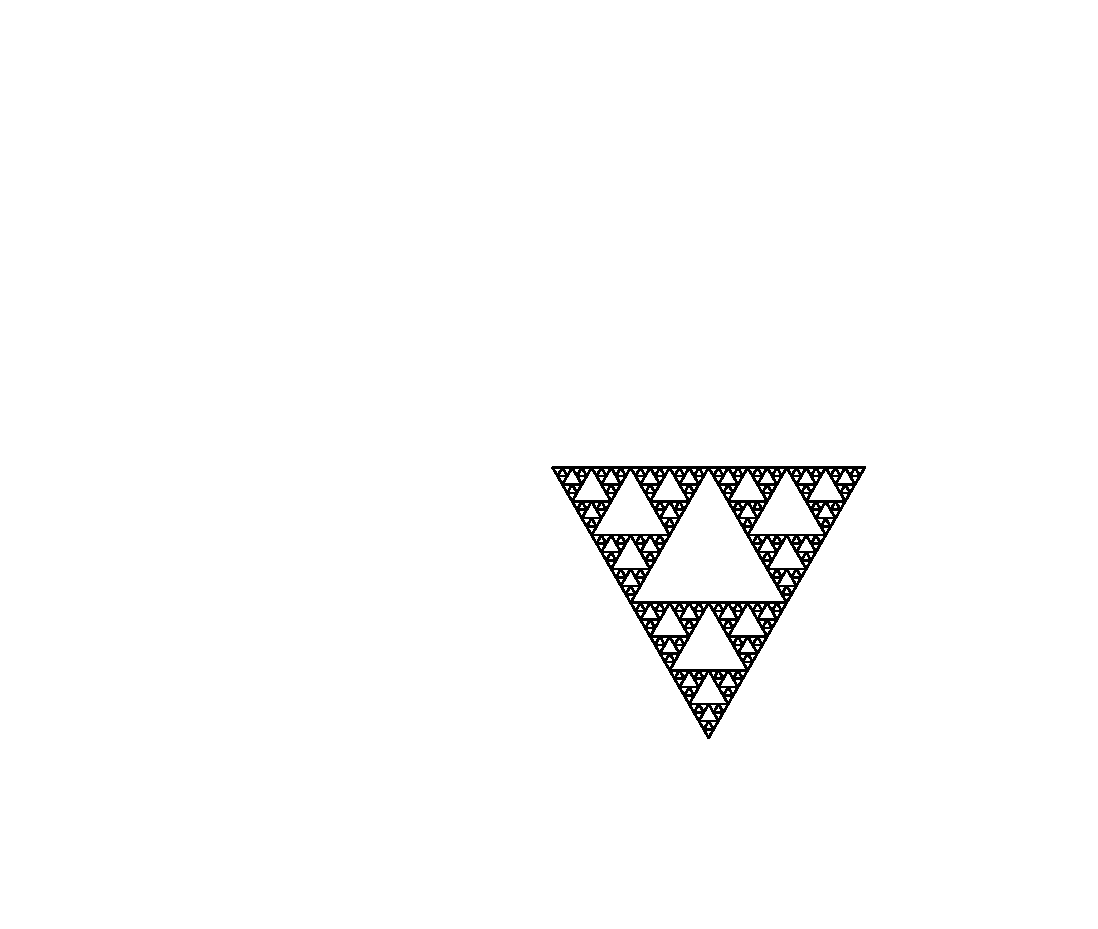
\includegraphics[width=0.6\textwidth]{triangle}
  \caption{Sierpinski triangle with 5 subdivisions.}
\end{figure}
Revisiting the initial code, the faultiness of its algorithm became apparent and hence could be corrected. The effectiveness of this new code compared to the approach recommended in the project description is due to the lack of redundant drawing. \par We used an iterative development process, meaning we started out by making a small piece of the code work in one iteration. Through testing, trial and error the goal of the iterative step was reached and we then carried on with the next step, where more code was implemented and tested. After several steps, we realized that our approach was overly complicated, so we started again from scratch. This time we did not care for optimization of the algorithm, and we solely focused on correctness.\footnote{The source code for this part of the project can be found in the file \href{https://github.com/ErikAndersen81/DM550-FractalProject/blob/master/sierpinsky-triangle.py}{sierpinsky-triangle.py}}
\begin{figure}[H]
  \centering
  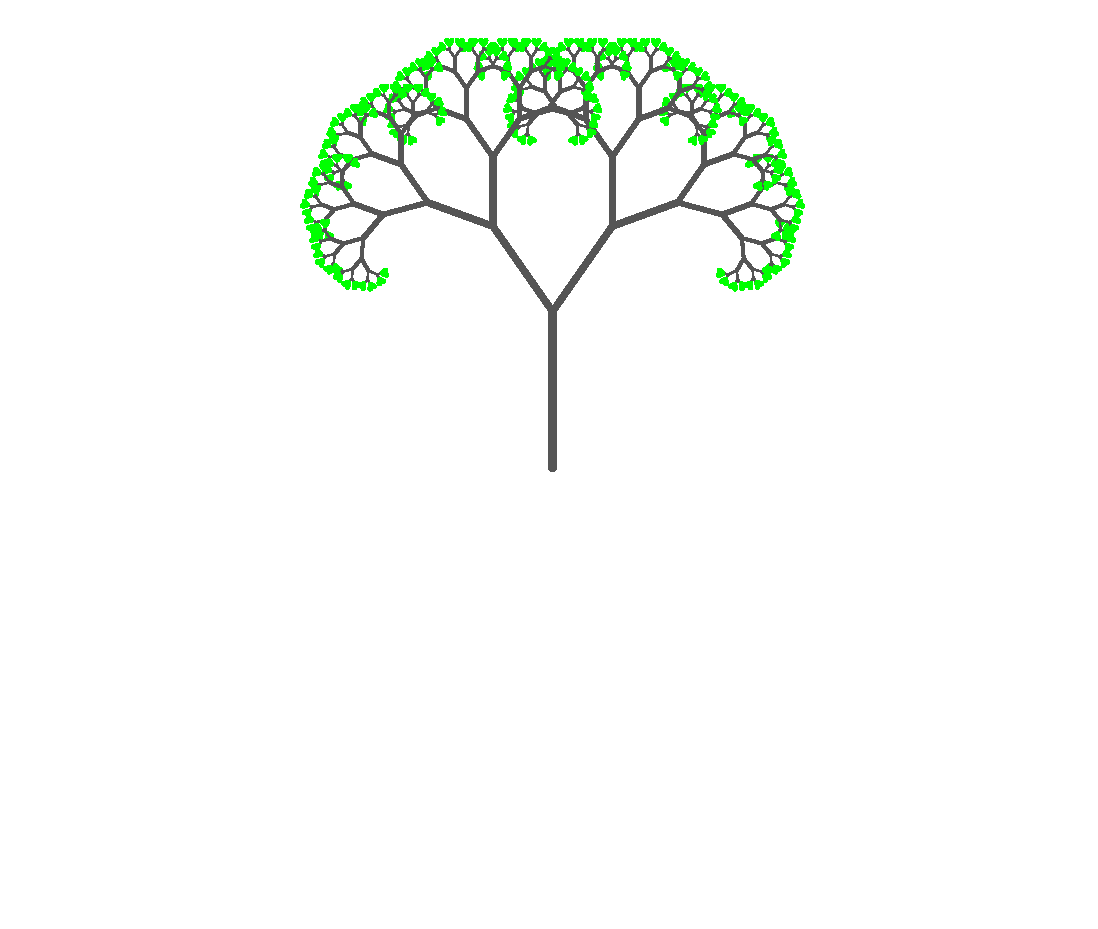
\includegraphics{bintree}
  \caption{Binary tree}
\end{figure}
section{Binary three}
\subsection{Specification and design}
We began by trying to define a function with two parameters (size, step)
\section{Fern}
First of all we define a function for the stem on the fern with several important parameters (length, width, segments curve, steps)
The segments are the number of branches on the fern. To demonstrate segments the for loop is necessary tool. The pensize is thickness of the leaves and for each step the pensize degrees with 0,3. The curve is the angle of the leaves and for each turn the angle degrees with 0,3. 
One of the interesting functions in python is the clone method. The idea with a clone method is too clone every time we turn left or right. The function calls itself with the parameters and the clone but this time the length and width degrees with 0,3 and the segments degrees with one step.
\section{FDL-Parser}
Since the fdl-file is to be read by an instance of the turtle module's Turtle class, it was decided to make a subclass of it called SmartTurtle. This class should be able to read a fdl-file, and execute he commands, giving a reasonable result. Through analyzis of several fdl-files, a decision as to which attributes the SmartTurtle class should implement could be made. Thus, an instance of the SmartTurtle should have a start command, a length, a depth, a dictionary of rules, and one of commands which could be called with appropriate arguments. The rules should be unfolded according to the depth of the smartturtle, so a unfolded attribute would be convenient. This attribute would initially be an empty string, but when the user of the SmartTurtle class would want to execute the commands in the fdl-file loaded, a function to unfold the rules list is required.  
\end{document}
